\subsection{Galaxy Photometry}
\label{sec:galaxy_photometry}

Galaxy photometry investigations so far have used the Extended Chandra Deep Field-South (ECDFS) due to the availability of public external reference data, including space-based imaging from the Hubble Space Telescope (HST).
Broadly, we have done (or soon will be doing) comparisons to matches against external catalogs and from synthetic source injection (SSI) in coadds.
Some preliminary investigations were done with visual inspection of external images.

\iffalse                                % doesn't appear to have added much to ComCam analysis
\subsubsection{Comparison to External Imaging}
\label{subsec:galaxy_photometry_external_imaging}

We downloaded a subset of the Hubble Legacy Fields (HLF, \url{https://archive.stsci.edu/prepds/hlf/}) imaging for the GOODS-South field, which included programs covering the original Chandra Deep Field-South and parallel fields now part of ECDFS.
Significantly overlapping coverage is available in F435W, F606W, F775W and F814W, as well as four redder bands.
F775W is of particular interest for galaxy photometry since it was designed to match the SDSS i-band filter.

Visual inspection of a particular group of photogenic galaxies in the HST imaging revealed an excess point source in the ComCam imaging from Nov. 8, which was subsequently found to match the position of an alert issued by several ZTF brokers in early September.
We experimented with using the HST image as a template for difference imaging by PSF matching and resampling to ComCam resolution.
This can be done relatively successfully on a per-object basis, but unfortunately, the image registration/warping for the HST images is too inconsistent to make it worthwhile on patch scales without re-warping one image or the other.

Besides visual inspection, no other uses of or comparisons to external imaging have yet been demonstrated.
DM-47576 (\url{https://rubinobs.atlassian.net/browse/DM-47576}) has been informally assigned to an in-kind contributor to make loading and displaying HST images more convenient should a need arise.

Joint modelling of space and ground imaging has been demonstrated with MultiProFit in COSMOS with the Subaru Hyper Suprime-Cam (HSC) and HST data on DM-46497 (\url{https://rubinobs.atlassian.net/browse/DM-46497}) but has not been attempted with ComCam data and is not considered a high priority, in part due to the aforementioned astrometry/warping issues.
\fi

\subsubsection{Comparison to External Catalogs}
\label{subsec:galaxy_photometry_external_catalogs}

DM-47234 (\url{https://rubinobs.atlassian.net/browse/DM-47234}) compared the tract 5063 20241120 DRP object table galaxy photometry with the latest HLF and Dark Energy Camera Legacy Survey DECaLS (DECaLS, \url{https://www.legacysurvey.org/decamls/}) catalogs.

\begin{figure}
  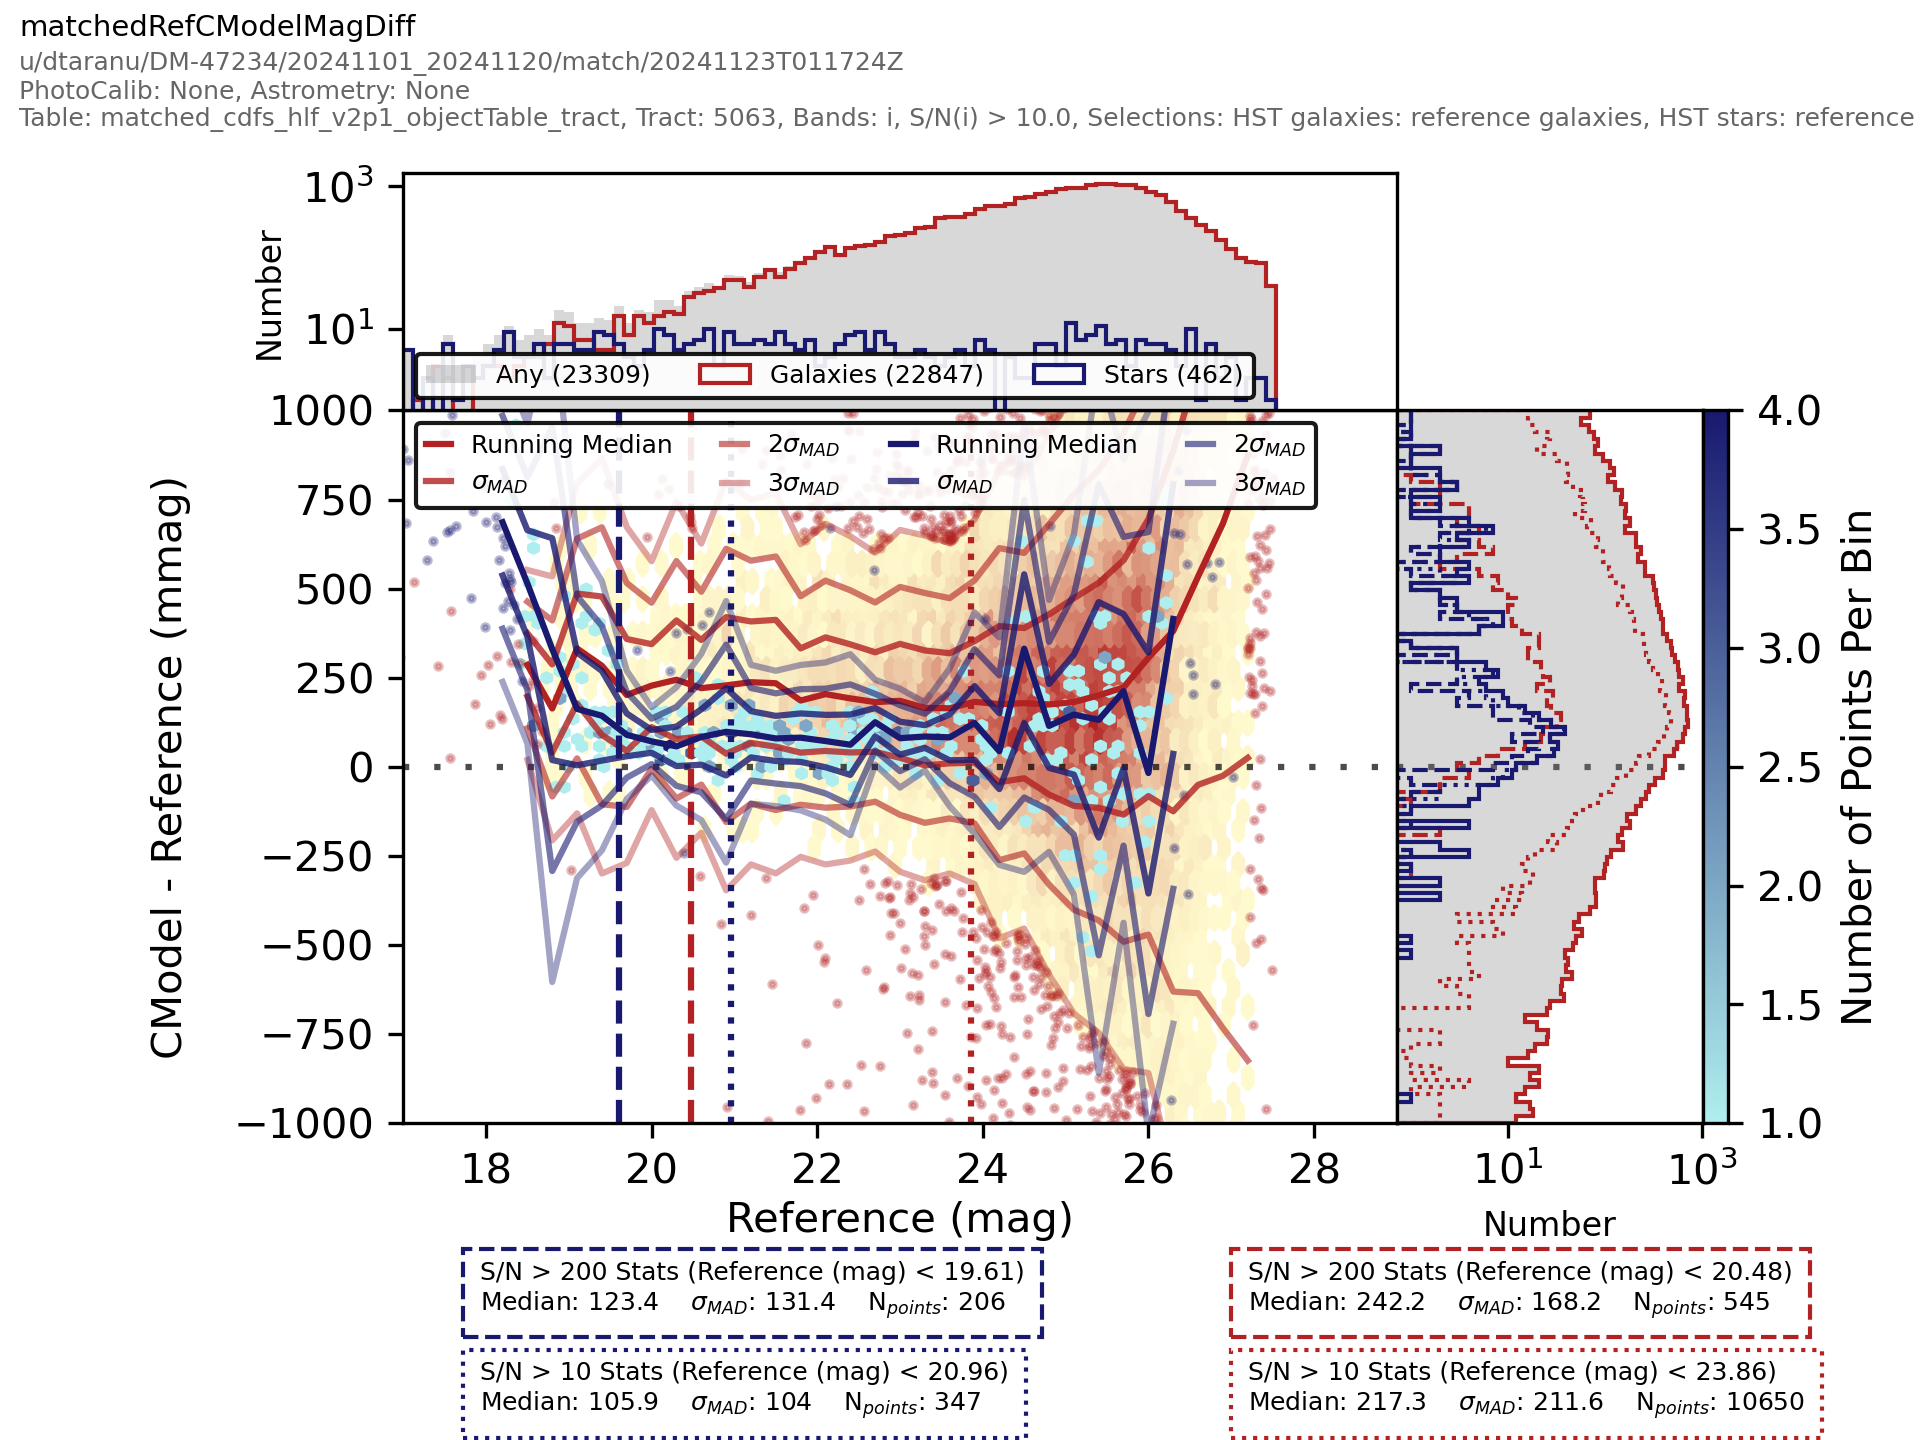
\includegraphics{galaxy_photometry/cdfs_i_vs_HST_F775W.png}
  \caption{Difference between i-band CModel magnitudes and HST F775W magnitudes in ECDFS.}
  \label{fig:cdfs_i_vs_HST_F775W}
\end{figure}

\figRef{cdfs_i_vs_HST_F775W} shows difference between i-band CModel magnitudes and the HLF HST F775W SourceExtractor magnitudes for both stars and galaxies, using the HST star-galaxy classification.
The median difference in both stellar and galaxy photometry is fairly flat across 19<i<25, but also quite large at about 175 mmag for galaxies and 75 mmag for stars.
Presuming that the difference in stellar photometry is mainly a calibration issue, the differential between galaxies and stars is still more than a factor of 2 (and still more in quadrature).
This could be due to differences in methodology; the HST SourceExtractor-derived magnitudes are more like aperture photometry than a model fit.

\begin{figure}
  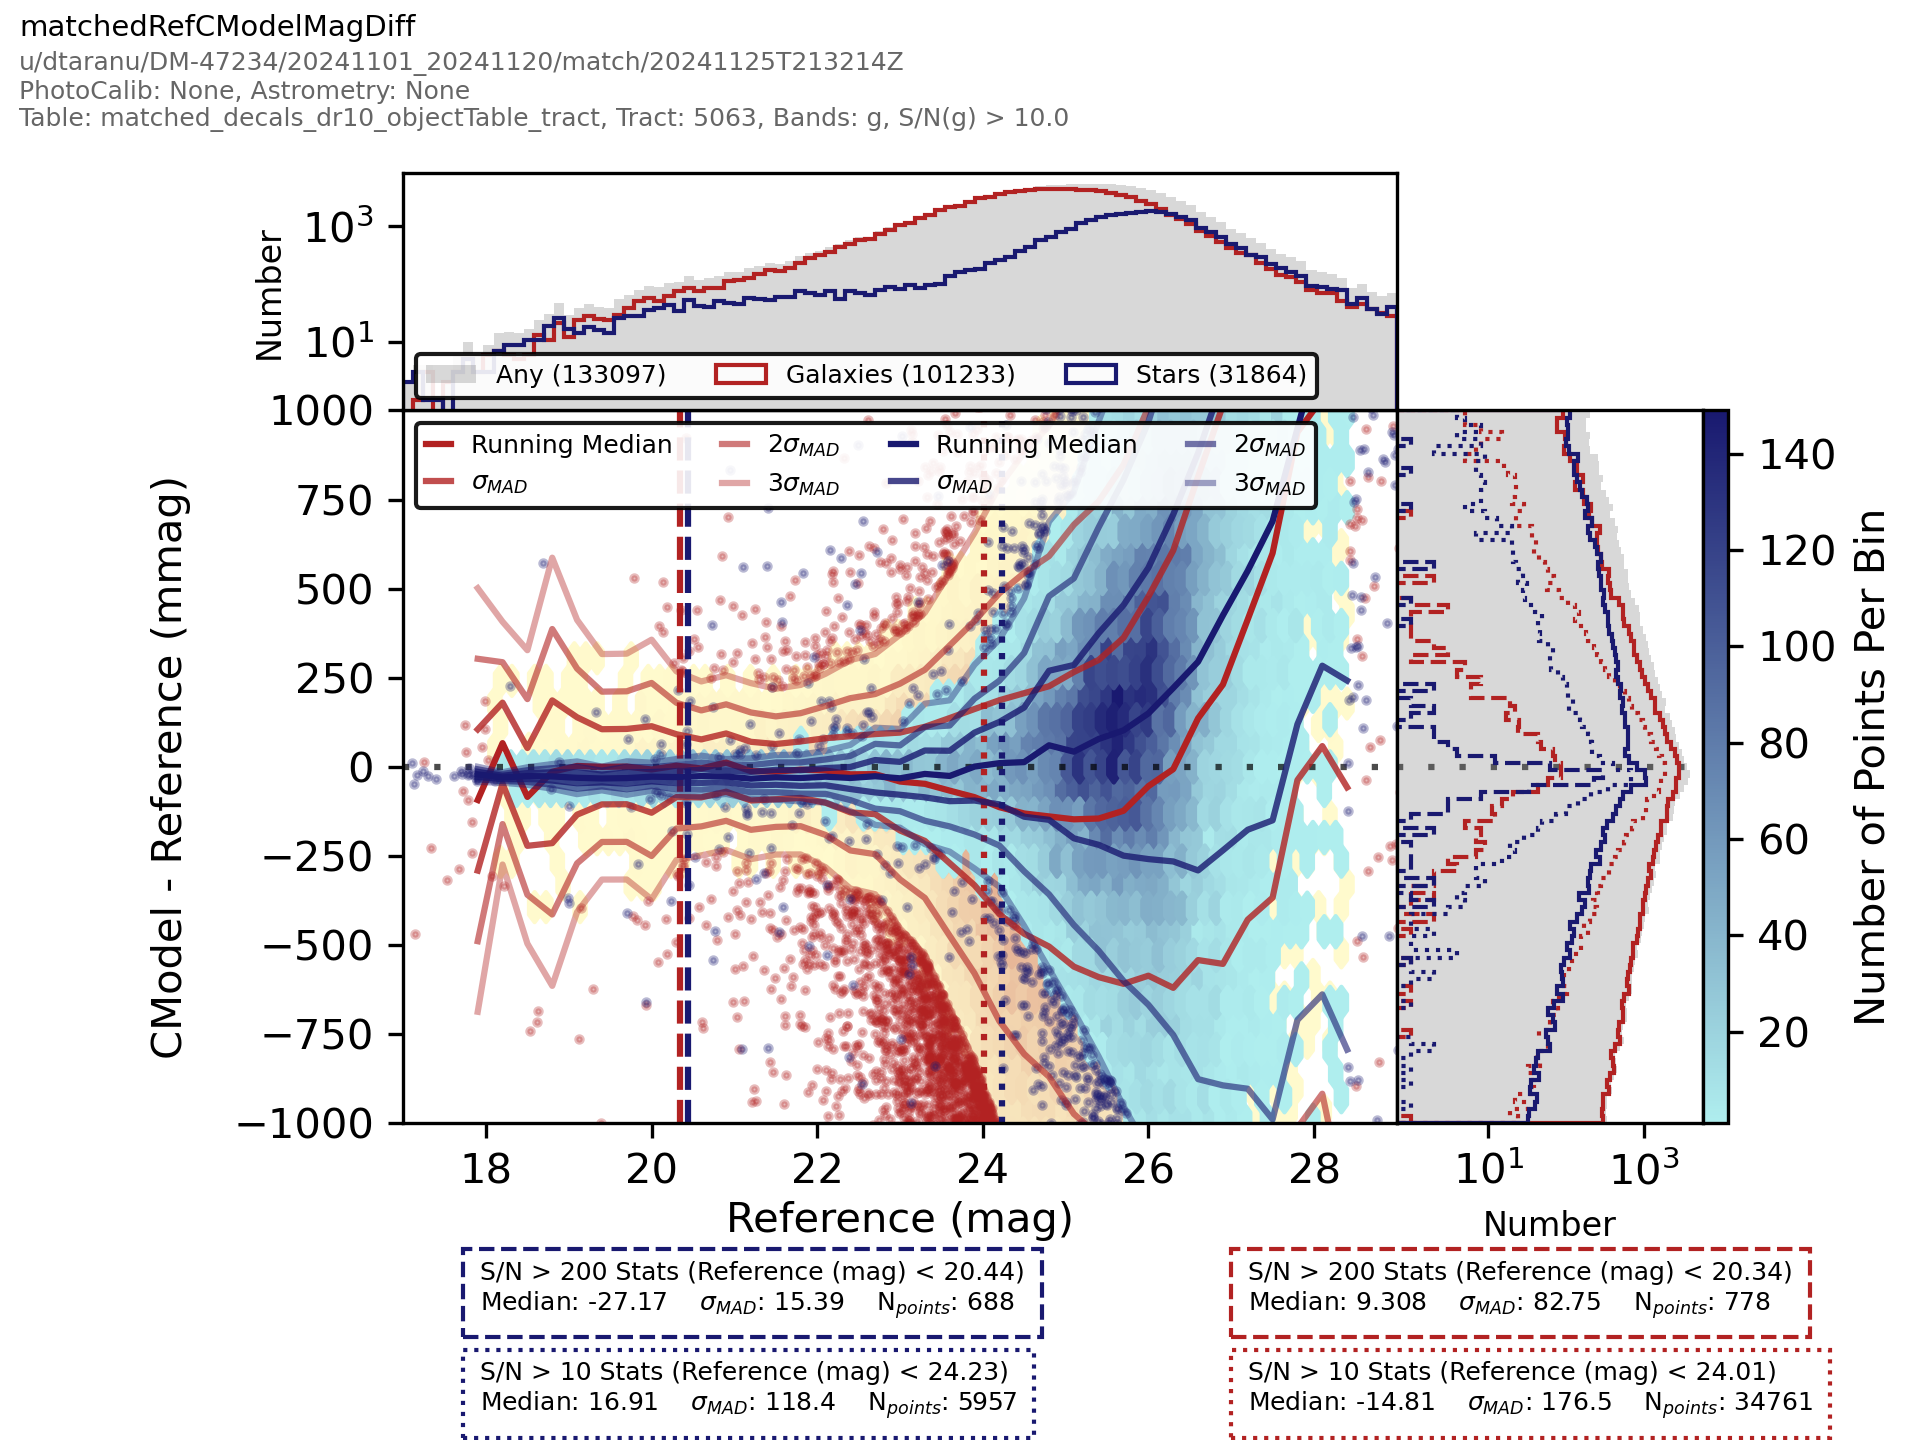
\includegraphics[width=0.5\textwidth]{galaxy_photometry/cdfs_g_vs_DECaLS.png}
  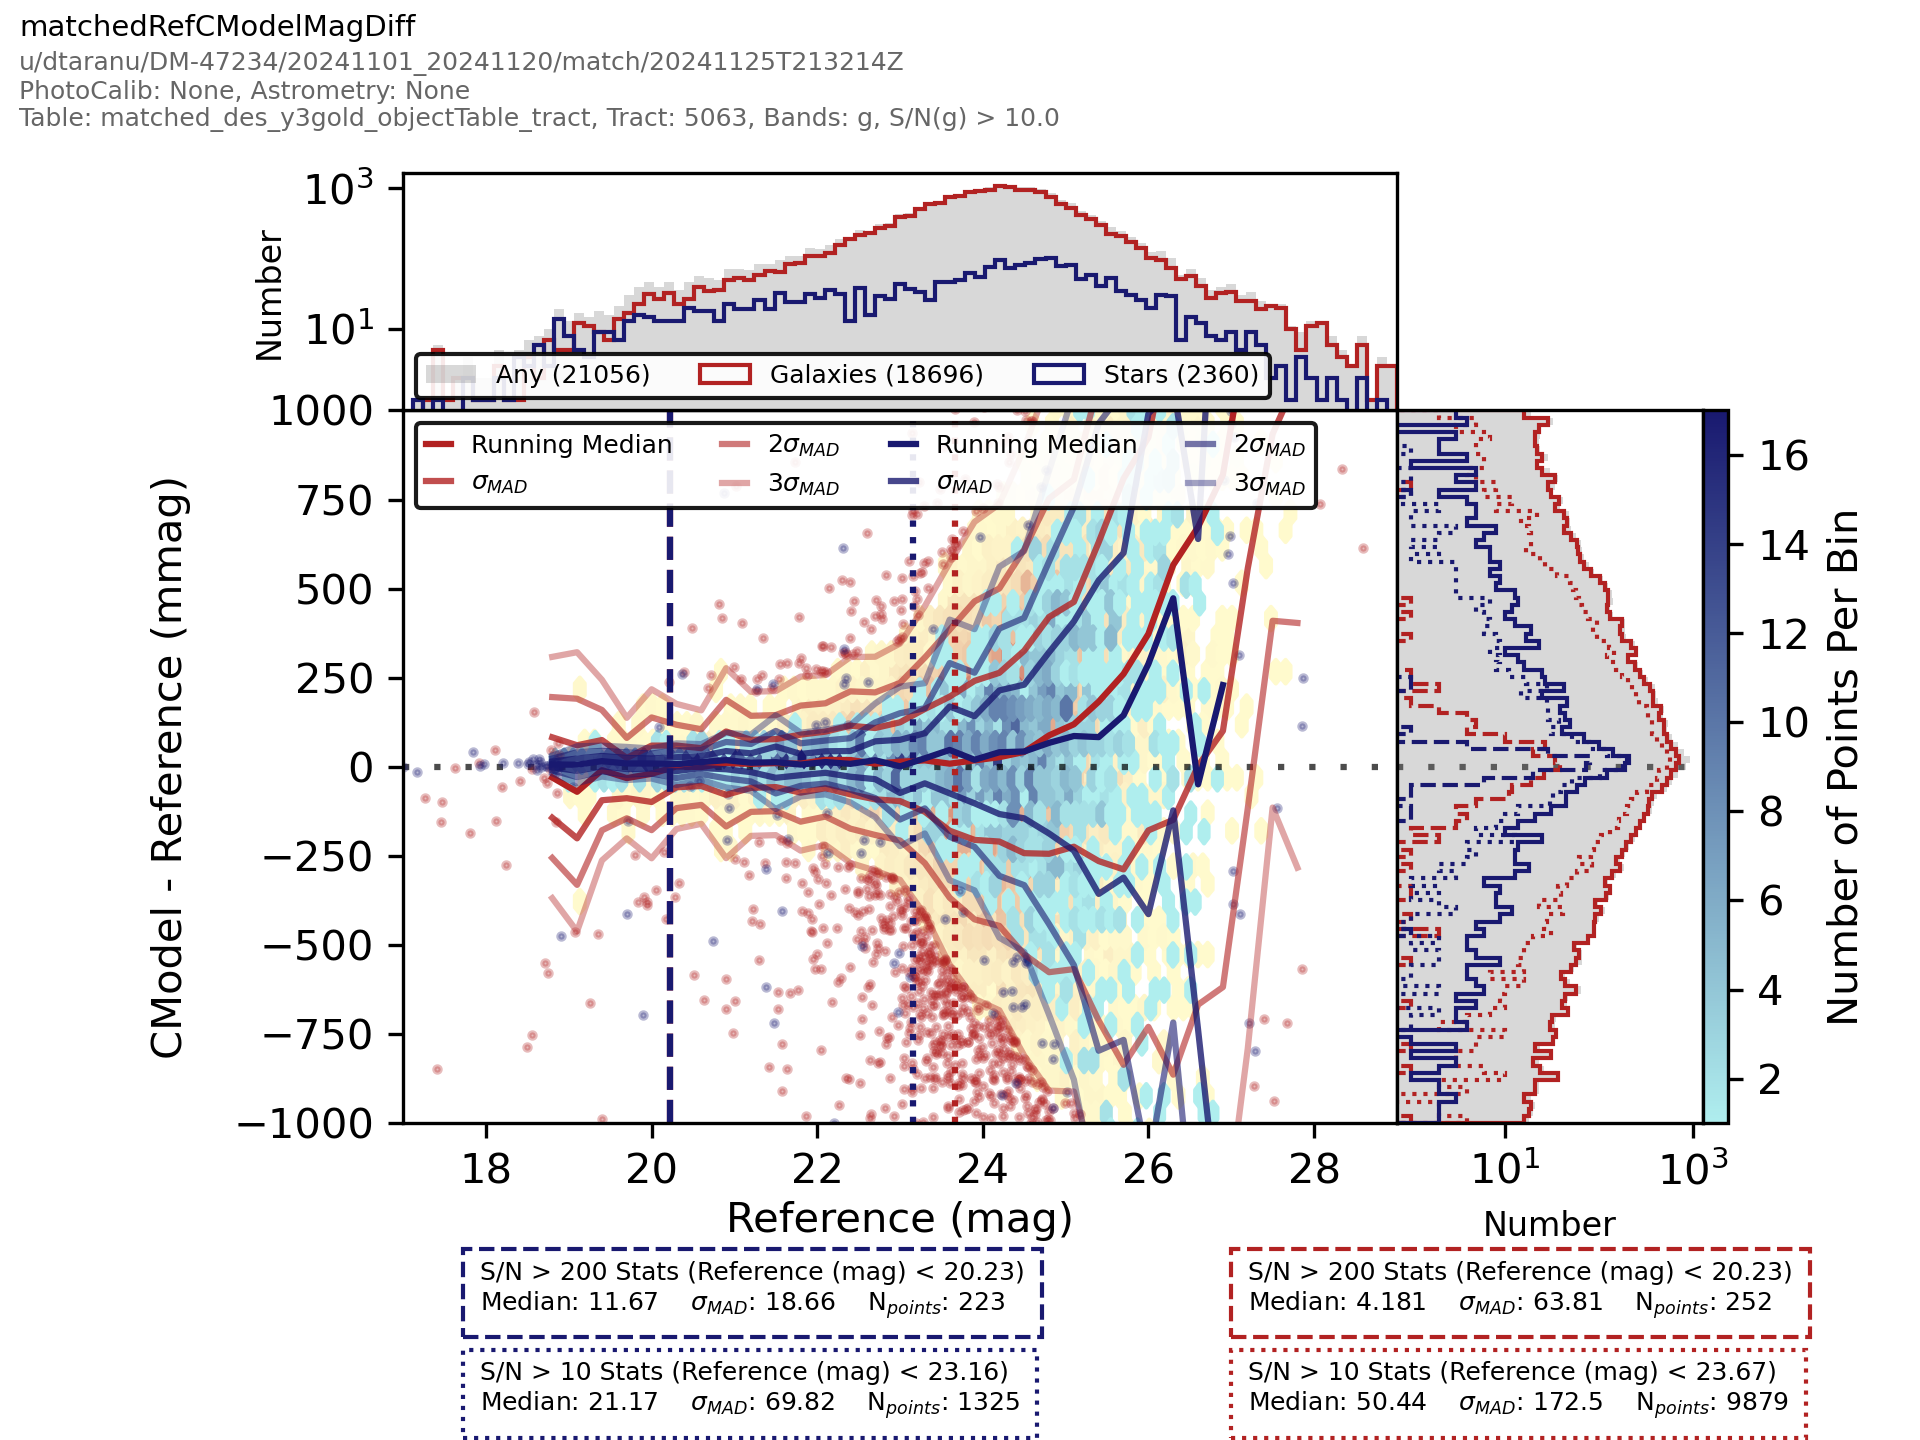
\includegraphics[width=0.5\textwidth]{galaxy_photometry/cdfs_g_vs_desy3g.png}
  \caption{Difference between g-band CModel magnitudes and DECaLS/DES-Y3G catalog values in ECDFS.}
  \label{fig:cdfs_g_vs_des}
\end{figure}

\figRef{cdfs_g_vs_des} shows the difference between g-band CModel magnitudes and measurements from two Dark Energy Survey (DES) DECam (Dark Energy Camera)-based catalogs.
The DECaLS (Dark Energy Camera Legacy Survey) DR10 processing is more recent and includes model photometry, selecting the least complicated model required to provide a good fit from a PSF to a single free Sersic fit.
The Dark Energy Survey Year 3 Gold (DES-Y3G) sample is an older, shallower dataset, albeit using pipelines more similar to the ComCam/DRP pipelines.
The median difference between stellar magnitudes is relatively small but varies with magnitude and between the two catalogs.
However, given the difference between filters and that no color term corrections have been applied, both the medians offset and scatter of 10 to 30 mmag are acceptable.
Bright ($g < 20.3$) galaxies have median offsets smaller than 10 mmag and scatter of 82 and 64 mmag in DECaLS and DES-Y3G, respectively.

\begin{figure}
  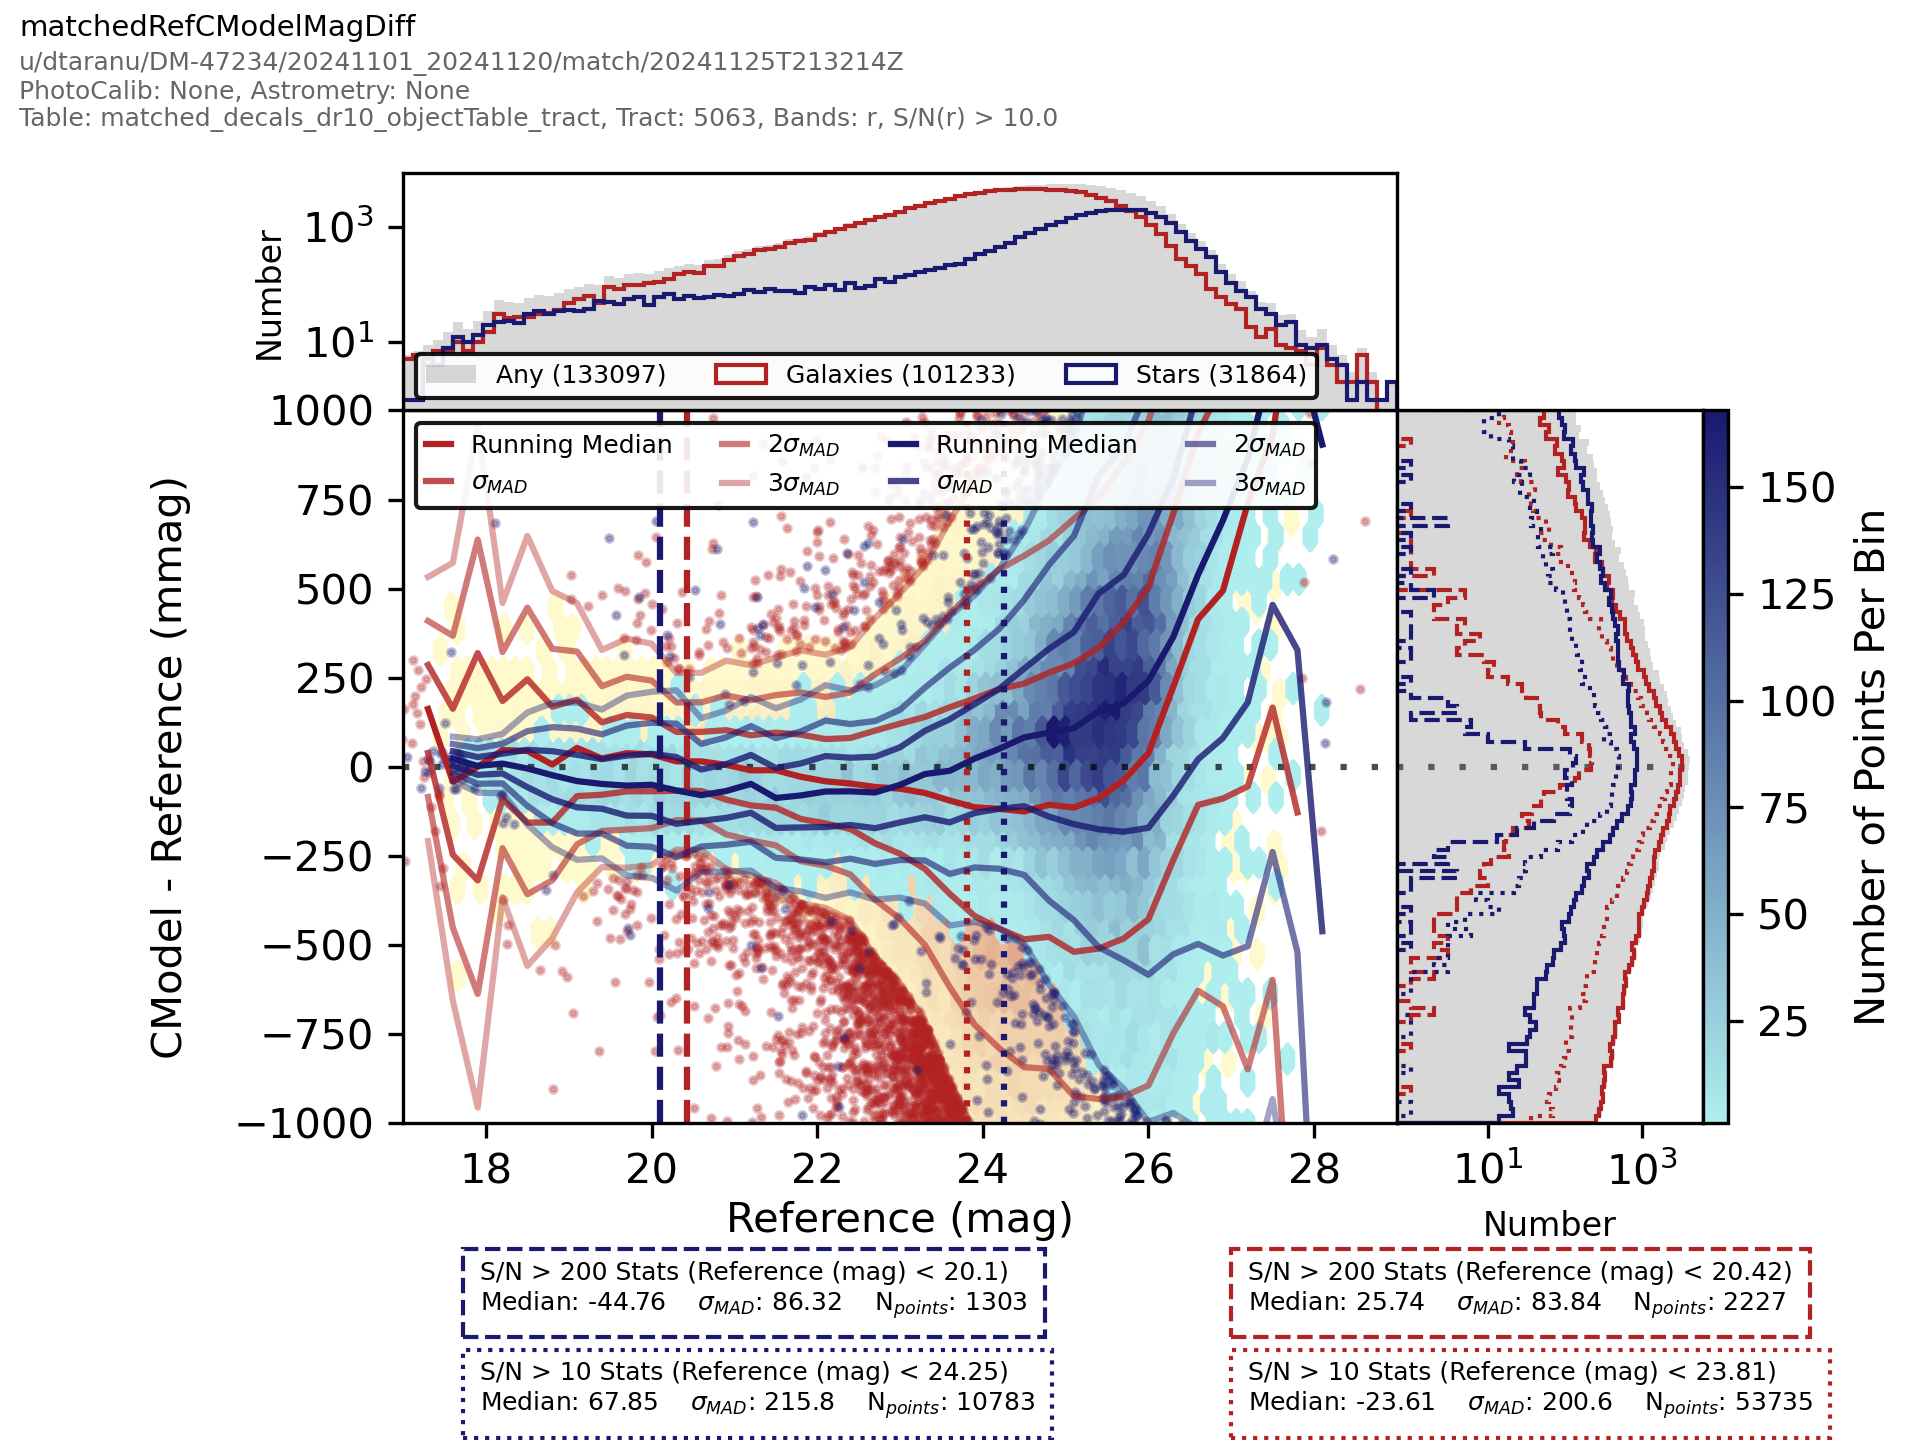
\includegraphics[width=0.5\textwidth]{galaxy_photometry/cdfs_r_vs_DECaLS.png}
  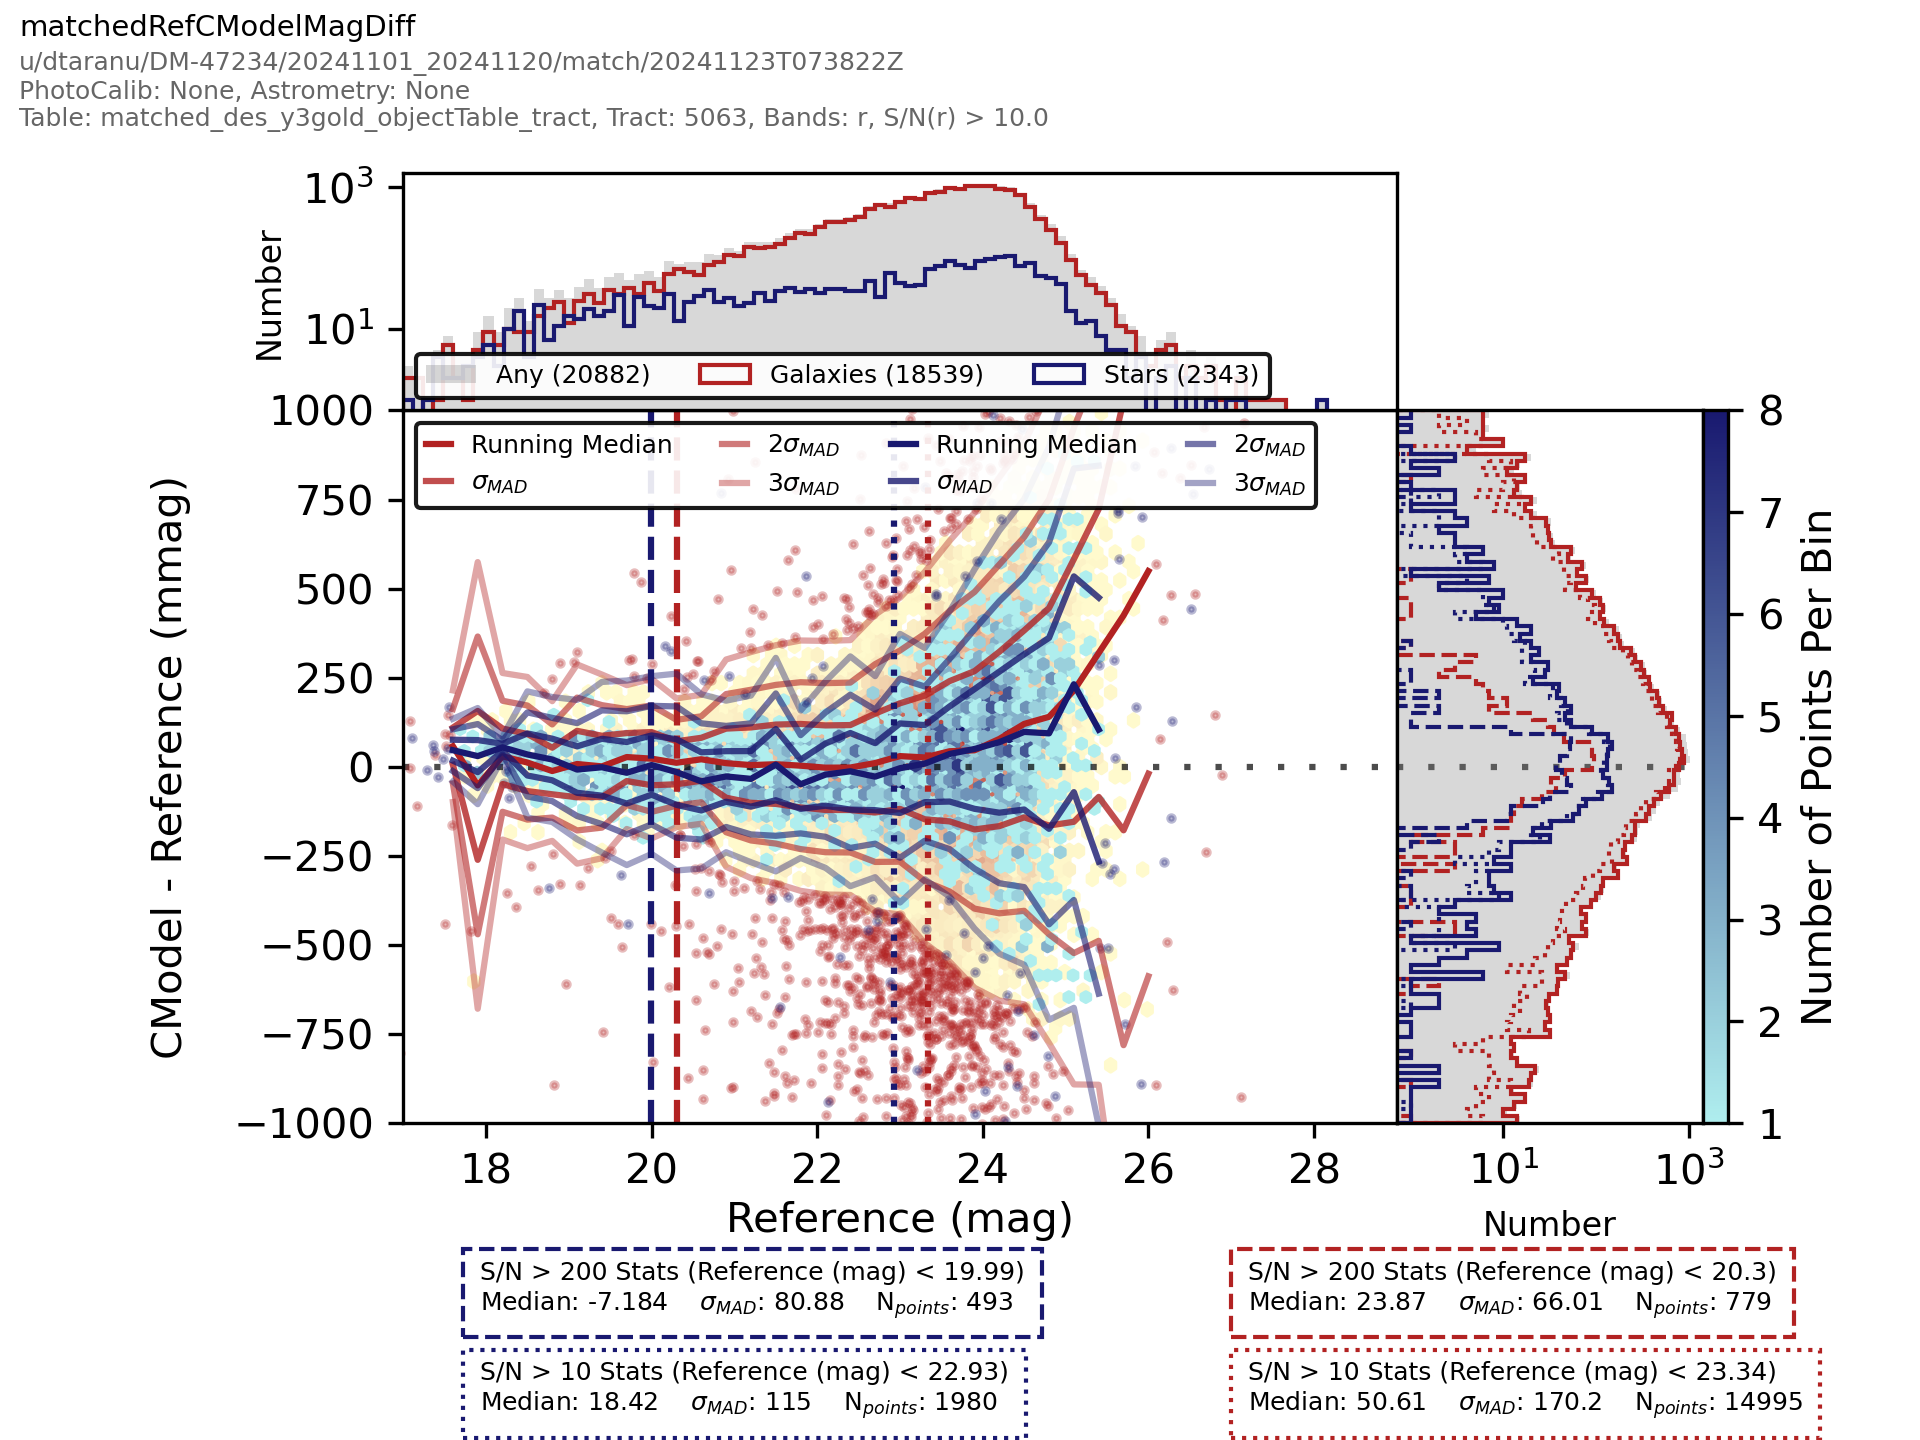
\includegraphics[width=0.5\textwidth]{galaxy_photometry/cdfs_r_vs_desy3g.png}
\caption{Difference between r-band CModel magnitudes and DECaLS/DES-Y3G catalog values in ECDFS.}
  \label{fig:cdfs_r_vs_des}
\end{figure}

\figRef{cdfs_r_vs_des} shows r-band magnitude difference plots.
Here, the median difference for stars are magnitude-dependent in both catalogs, suggesting that color terms are more important.
Similarly, the scatter is much larger, at about 80mmag for $r < 20$.
However, the magnitude dependence in the median difference is stronger in DECaLS, both for stars and galaxies.
Inspection of the $g-r$ versus $r-i$ stellar locus plot (not shown) reveals that DECaLS photometry has a substantial fraction (about 10\%) of outliers, some even a full magnitude off the stellar locus.
At any rate, the scatter in galaxy magnitudes is not much larger than that for stars (in fact, it is noticeably smaller in DES-Y3G).
Additionally, in DES-Y3G, the median magnitude difference is fairly flat for $19<r<23$, so despite the numerous differences in hardware and software, the two catalogs are not inconsistent.
The i-band photometry in DECaLS shows qualitatively similar but quantitatively worse pathologies and is omitted for brevity.

\begin{figure}
  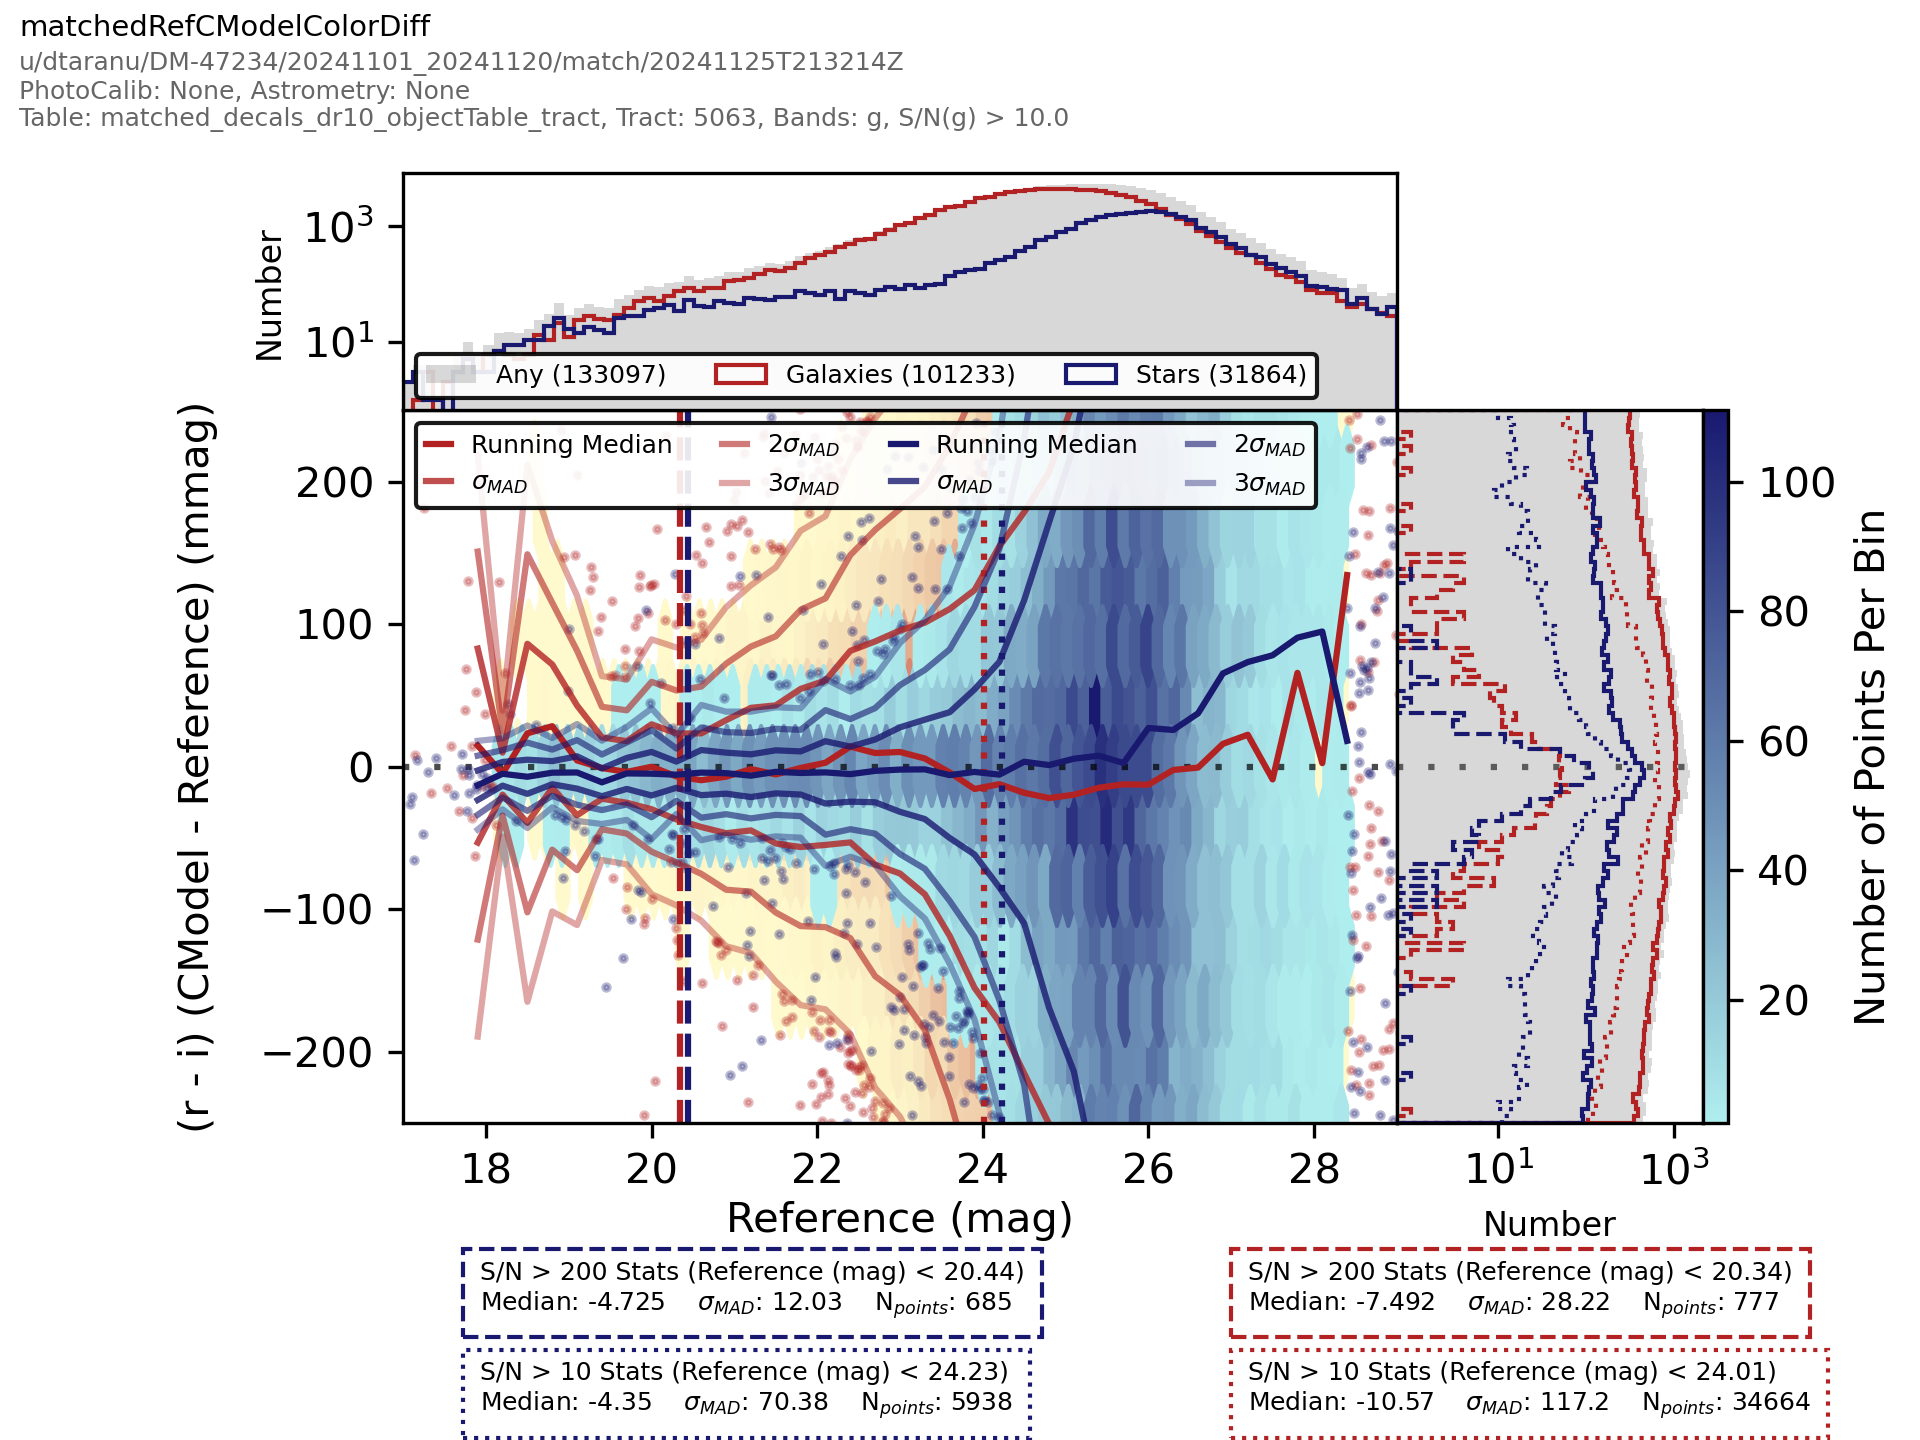
\includegraphics[width=0.5\textwidth]{galaxy_photometry/cdfs_g_vs_rmi_DECaLS.png}
  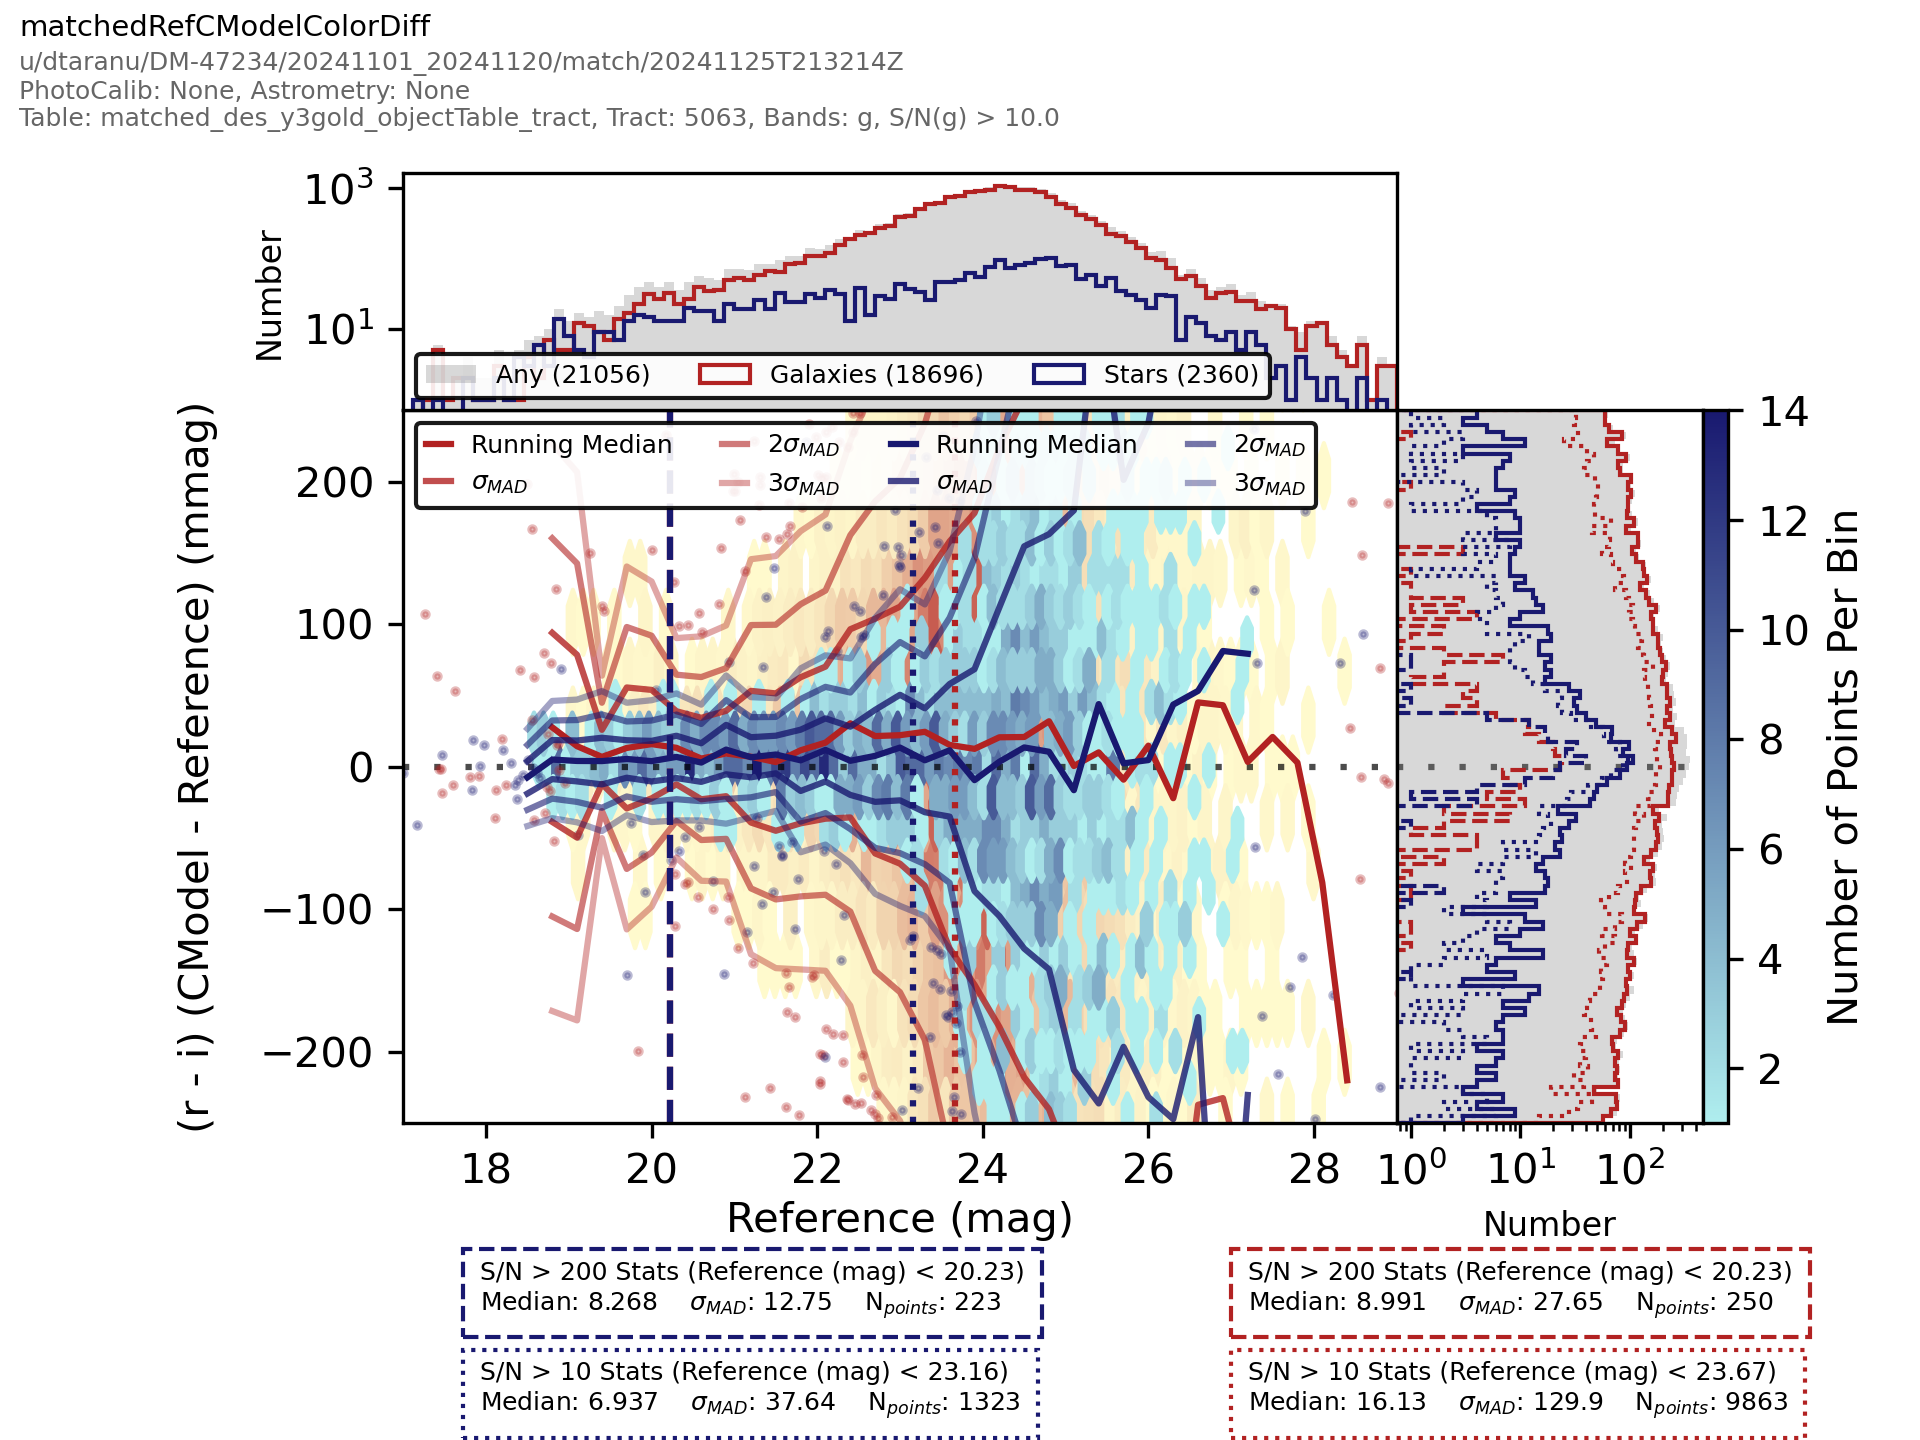
\includegraphics[width=0.5\textwidth]{galaxy_photometry/cdfs_g_vs_rmi_desy3g.png}
\caption{Difference between $r-i$ CModel colors and DECaLS/DES-Y3G catalog values in ECDFS.}
  \label{fig:cdfs_rmi_vs_des}
\end{figure}

The $r-i$ color differences shown in \figRef{cdfs_rmi_vs_des} are similar between all three catalogs.
The median differences are very small, albeit different in sign between the two pairs of catalogs.
The scatter in star color differences is nearly constant to about 22nd magnitude, whereas for galaxies it scales with signal-to-noise to a minimum of about 25mmag at 20th mag (photometry for brighter galaxies is limited by model inadequacy and irregular structure).
In short, galaxy colors appear quite consistent between all three catalogs, although how the small differences impact derived quantities like photometric redshifts remains to be seen.

\subsubsection{Additional Investigations}
\label{subsec:galaxy_photometry_additional}

Analysis of the accuracy of magnitude and color errors await the implementation of synthetic galaxy injection in DM-47185 (\url{https://rubinobs.atlassian.net/browse/DM-47185}).
Some analysis is possible with matching to reference catalogs; however, besides the problems with the DECaLS photometry, we are not yet taking into account reported errors on reference fluxes (which may themselves be underestimated).

Besides single-band/forced CModel photometry, MultiProFit multi-band (gri) single Sersic fits have been run on a single patch in tract 5063 on DM-47526 (\url{https://rubinobs.atlassian.net/browse/DM-47526}) but have yet to be analyzed.
Other algorithms like aperture, GaAP and Kron magnitudes/colors have yet to be compared.

\subsubsection{Conclusions}
\label{subsec:galaxy_photometry_conclusions}

Galaxy photometry in ECDFS appears consistent with at least two different catalogs covering the same field (one space based) and the differences identified in a third (DECaLS) appear to be peculiar to that catalog, not our own processing.
This is not to say that the galaxy photometry is optimal, as hardware and software differences make it difficult to quantify expected differences.
Comparisons to external data should be more illuminating once we have coadds in the COSMOS field and can compare to HSC imaging with the same pipeline versions.
